
%! Author = lili
%! Date = 7/25/26



\chapter{Schließende Statistik: Testtheorie I}\label{ch:schlieende-statistik:-testtheorie-i}

\noindent \textbf{Ziel:} Schließen von einer Stichprobe auf Verteilungsparameter.


\section*{Annahme}
Im Folgenden nehmen wir stets an, dass eine Stichprobe $x_1,\dots,x_n$ vorliegt, von der wir annehmen können, dass
sie aus Werten besteht, die von einem $n$-fach unabhängig wiederholten Zufallsexperiment stammen.

Das heißt, wir nehmen an, dass es einen Wahrscheinlichkeitsraum $\wraum$, unabhängige, identisch verteilte, $\rz$
-wertige Zufallsvariablen $X_1,\dots,X_n$ und ein $\ele\in\eraum$ gibt derart, dass
\[
    (x_1,\dots,x_n) = (X_1(\ele),\dots,X_n(\ele)) \cdot
\]
Wir werden die Theorie jeweils am Beispiel von \gls{Bernoulli-Variable}n illustrieren.

\begin{bsp}[Fragestellung im Fall von \gls{Bernoulli-Variable}n]
    \txc{(Skript 26)} \\
    Die $n$ unabhängigen \gls{Bernoulli-Variable}n können wir als Modell verstehen für das Werfen einer (nicht
    unbedingt fairen) Münze, für das Werfen einer Reißzwecke oder auch für einen Spezialfall des Werfens unserer
    Schweinchen: Beim Werfen der Schweinchen in der Vorlesung haben wir die Schweinchen 166-mal geworfen.
    Wenn wir nur jene Würfe als Erfolg gezählt hätten, in denen ein Schweinchen auf der Schnauze gelandet ist, so
    wäre dies ein Bernoulli-Experiment gewesen.
    Wir können jedoch auch im Nachhinein die anderen Resultate ignorieren und unser Experiment als reines
    Bernoulli-Experiment betrachten, wenn uns nur eine der möglichen Positionen interessiert.

    All diesen Situationen ist gemein, dass wir die tatsächliche Erfolgswahrscheinlichkeit nicht kennen und auch
    kein Symmetrieargument verwenden können, um diese zu bestimmen.
    Wir arbeiten daher zunächst mit einem Parameter, der in der Statistik üblicherweise mit $\theta$ bezeichnet wird
    und die Rolle der Erfolgswahrscheinlichkeit übernimmt.

    Im Fall von \gls{Bernoulli-Variable}n ist das Modell für das Zufallsexperiment also gegeben durch
    \begin{itemize}
        \item Ereignisraum $\eraum=\{0,1\}^n$
        \item unbekannte Erfolgswahrscheinlichkeit $\theta\in[0,1]$
        \item Wahrscheinlichkeitsfunktion $\wfk_\theta(\ele) = \theta^{\sum_{i=1}^n \ele_i}(1-\theta)^{n-\sum_{i=1}^n\ele_i}$ für alle $\ele\in\eraum$
        \item $X_i:\eraum\to\{0,1\}$ mit $X_i(\ele)=\ele_i$ für alle $\ele\in\eraum$ und alle $i\in\{1,\dots,n\}$
    \end{itemize}
\end{bsp}

\begin{defi}[Stichprobe, Stichprobenvariable und Stichprobenraum]
    \txc{(Skript 26)}
    \begin{enumerate}[label=(\alph*)]
        \item Die Zufallsvariablen $X_1,\dots,X_n$ heißen \emph{Stichprobenvariable}.
        \item Eine Realisation
        \[
            x = (x_1,\dots,x_n) = (X_1(\ele),\dots,X_n(\ele)) = X(\ele)
        \]
        für ein gegebenes $\ele\in\eraum$ heißt \emph{Stichprobe}.
        \item Der Bildbereich $\mathcal{X} = X(\eraum) = (X_1,\dots,X_n)(\eraum)$ der $n$-dimensionalen Zufallsvariablen $X$ heißt \emph{Stichprobenraum}.
        Der \gls{Stichprobenraum} $\spr$ ist die Menge aller möglichen Stichproben (bei gegebenem Experiment).
    \end{enumerate}
\end{defi}

\begin{bsp}[\gls{Bernoulli-Variable}]
    \txc{(Skript 26)} \\
    Im Fall von \gls{Bernoulli-Variable}n erfüllen die unabhängigen \gls{Stichprobenvariable}n $X_1,\dots,X_n$
    \[
        \pe_{\theta}(X_i=1)=\theta \qquad\text{und}\qquad \pe_{\theta}(X_i=0)=1-\theta \qquad \forall i\in\{1,\dots,n\} \cdot
    \]
    Ist $n=3$ und $\ele\in\eraum$ zum Beispiel gegeben durch $\ele=(0,0,1)$, so ergibt sich die Stichprobe zu $x=(x_1,x_2,x_3)=(X_1(\ele),X_2(\ele),X_3(\ele))=(0,0,1)$, weil die \gls{Stichprobenvariable}n in diesem Fall die Projektionen von $\eraum$ auf die einzelnen Komponenten sind.

    Der \gls{Stichprobenraum} ist $\spr = X(\eraum) = \{0,1\}^3$.
\end{bsp}

\begin{defi}[Statistisches Modell]
    \txc{(Skript 26)} \\
    Ein \emph{statistisches Modell} für ein gegebenes Zufallsexperiment ist eine Familie $\pefam$ von
    Wahrscheinlichkeitsmaßen $\pe$ auf dem \gls{Stichprobenraum} $\spr$, wobei die Wahrscheinlichkeitsmaße $\pe \in\pefam$ die möglichen Verteilungen von $X=(X_1,\dots,X_n)$ beschreiben.

    Gilt $\pefam = \{\pe_{\param} : \param\in\praum\}$, so heißt $\praum$ der \emph{Parameterraum} und $\param\in\praum$ heißt \emph{Parameter}.
\end{defi}

\begin{bsp}[\gls{Bernoulli-Variable}]
    \txc{(Skript 26)} \\
    Im Fall von unabhängigen \gls{Bernoulli-Variable}n als \gls{Stichprobenvariable} $X_1,\dots,X_n$ ist das zugehörige statistische Modell gegeben durch $\pefam = \{\pe_{\param}:\param\in\praum\}$, wobei wir im Allgemeinen $\praum=[0,1]$ wählen und $\pe_{\param}$ durch die Wahrscheinlichkeitsfunktion $\wfk_\param$ mit
    \[
        \wfk_\param(\ele) = \param^{\sum_{i=1}^n\ele_i}(1-\param)^{n-\sum_{i=1}^n\ele_i} \qquad \text{für alle } \ele\in\eraum
    \]
    gegeben ist.

    Wenn wir Grund haben anzunehmen, dass für die Erfolgswahrscheinlichkeit gewisse Werte ausgeschlossen werden können, so kann $\praum$ auch als echte Teilmenge von $[0,1]$ gewählt werden.
\end{bsp}

Unser Ziel ist es nun, systematisch aus Stichproben Schlüsse zu ziehen über die dem Zufallsexperiment zugrunde liegende Wahrscheinlichkeitsverteilung.
Konkreter heißt das: Wir nehmen an, dass wir die Verteilung der \gls{Stichprobenvariable}n bis auf den oder die
Parameter der Verteilung kennen, und wollen nun anhand einer Stichprobe die Parameter der Verteilung bestmöglich schätzen.
Im Fall von \gls{Bernoulli-Variable}n heißt das, dass wir die Erfolgswahrscheinlichkeit $\param$ schätzen wollen.
Im Folgenden werden wir auch andere Kennzahlen der Wahrscheinlichkeitsverteilung wie Erwartungswert oder Varianz schätzen.

Grundsätzlich gibt es verschiedene Typen von Resultaten, die wir anhand einer Stichprobe gewinnen können:
\begin{enumerate}
    \item \textbf{\gls{Punktschätzer}:} Resultat ist ein Wert $\param$ oder $g(\param)$ mit $\param\in\praum$
    \item \textbf{\gls{Bereichsschätzer}:} Resultat ist eine Teilmenge von $\praum$
    \item \textbf{\gls{Hypothesentest}:} Resultat ist eine Ja-Nein-Entscheidung über eine den Parameter betreffende \gls{Hypothese}
\end{enumerate}
Wir befassen uns in diesem Kapitel mit \gls{Punktschätzer}n.

\begin{defi}[\gls{Punktschätzer}]
    \txc{(Skript 26)} \\
    Sei ein statistisches Modell der Form $\pefam=\{\pe_{\param}:\param\in\praum\}$ gegeben.
    \begin{enumerate}[label=(\alph*)]
        \item Ein \emph{\gls{Schätzer}} für $\param\in\praum$ ist eine Abbildung $t:\spr\to\praum$.
        Wir nennen auch die Zufallsvariable $T=t(X)=t((X_1,\dots,X_n))$ einen \gls{Schätzer} für $\param\in\praum$.
        Eine Realisierung $t(x)=t((x_1,\dots,x_n))$ bzw.\ $T(\ele)$ heißt \emph{Schätzung} für $\param$.
        \item Sei zusätzlich eine Abbildung $g:\praum\to\Gamma$ gegeben.
        Ein \emph{\gls{Schätzer}} für $g(\param)$ ist eine Abbildung $t:\spr\to\Gamma$.
        Wir nennen auch die Zufallsvariable $T=t(X)=t((X_1,\dots,X_n))$ einen \gls{Schätzer} für $g(\param)$.
        Eine Realisierung $t(x)=t((x_1,\dots,x_n))$ bzw.\ $T(\ele)$ heißt \emph{Schätzung} für $g(\param)$.
    \end{enumerate}
    Wir werden uns zunächst auf \gls{Schätzer} für $\param$ konzentrieren und später auf \gls{Schätzer} für $g(\param)$ zurückkommen.
\end{defi}

\begin{bem}[Unterschied zwischen \gls{Schätzer} und Schätzung für $\param$]
    \begin{mytable}
        \begin{tabular}{ll}
            \hline
            \textbf{\gls{Schätzer} (Funktion)}        & \textbf{Schätzung (Funktionswert)} \\
            \hline
            Rechenvorschrift $t:\spr\to\praum$; & Ergebnis $t(x)$ der Auswertung     \\
            ordnet jeder Stichprobe einen             & der Rechenvorschrift für eine      \\
            Parameterwert zu                          & konkrete Stichprobe                \\
            \hline
        \end{tabular}
    \end{mytable}
\end{bem}

\begin{bsp}[\gls{Schätzer} können absurd schlecht sein]
    \txc{(Skript 26)} \\
    Im Fall von unabhängigen \gls{Bernoulli-Variable}n als \gls{Stichprobenvariable} $X_1,\dots,X_n$ haben wir den \gls{Stichprobenraum} $\spr=\{0,1\}^n$ sowie den Parameterraum $\praum=[0,1]$.
    Gemäß Definition ist die Abbildung $t:\spr\to\praum$ mit $t(x)=\frac12$ für alle $x\in\spr$ eine zulässige Wahl für einen \gls{Schätzer} der Erfolgswahrscheinlichkeit.
    Offensichtlich ist diese, nicht von der Stichprobe abhängige Wahl nicht sinnvoll.

    Motiviert durch das Gesetz der großen Zahlen und die Tatsache, dass für \gls{Bernoulli-Variable} der Erwartungswert der Erfolgswahrscheinlichkeit entspricht, vermuten wir, dass das arithmetische Mittel der Stichprobenwerte $t(x)=\frac1n\sum_{i=1}^n x_i$ eine klügere Wahl sein sollte.

    Dies wirft die Frage auf, wann ein \gls{Schätzer} ein guter \gls{Schätzer} ist.
    Wir benötigen Kriterien, um \gls{Schätzer} systematisch beurteilen zu können.
\end{bsp}

\begin{defi}[Kriterien zur Beurteilung von \gls{Punktschätzer}n]
    \txc{(Skript 26)} \\
    Gegeben seien ein statistisches Modell der Form $\pefam=\{\pe_{\param}:\param\in\praum\}$, eine Abbildung $g:\praum\to\Gamma$, sowie ein \gls{Schätzer} $t:\spr\to\Gamma$ für $g(\param)$.\footnote{Der Fall, dass wir mit einem \gls{Schätzer} für den Parameter $\param$ selbst arbeiten, entspricht der Wahl $\Gamma=\praum$ und $g(x)=x$ für alle $x\in\spr$. Wir müssen daher die beiden Fälle nicht unterscheiden.}

    \begin{enumerate}[label=(\alph*)]
        \item Der \emph{Bias} des \gls{Schätzer}s $t$ ist definiert als
        \[
            \mathrm{Bias}_t(\param) = \ET[T] - g(\param) = \ET[t((X_1,\dots,X_n))] - g(\param) \qquad \text{für alle } \param\in\praum \cdot
        \]
        Dabei sei $\ET$ der Erwartungswert, der mit dem Wahrscheinlichkeitsmaß $\pe_{\param}$ definiert ist.
        \item Der \gls{Schätzer} $t$ heißt \emph{erwartungstreu}, wenn $\mathrm{Bias}_t(\param)=0$ für alle $\param\in\praum$ gilt.
        \item Das \emph{Risiko} des \gls{Schätzer}s $t$ im Punkt $\param\in\praum$ ist definiert als die erwartete quadratische Abweichung des \gls{Schätzer}s von $g(\param)$, das heißt,
        \[
            R(\param,t) = \ET\big[(T-g(\param))^2\big] \cdot
        \]
        \item Die \emph{Risikofunktion} des \gls{Schätzer}s $t$ ist definiert als die Abbildung $\param\mapsto R(\param,t)$.
        \item Sind $t_1,t_2:\spr\to\Gamma$ zwei \gls{Schätzer} für $g(\param)$, so sagen wir, dass $t_1$ \emph{mindestens so gut} ist wie $t_2$, wenn $R(\param,t_1)\leq R(\param,t_2)$ für alle $\param\in\praum$ gilt.
        Gilt zusätzlich, dass es ein $\param\in\praum$ gibt mit $R(\param,t_1)<R(\param,t_2)$, so sagen wir, dass $t_1$ \emph{besser} als $t_2$ ist.
    \end{enumerate}
\end{defi}

\begin{bsp}
    \textbf{Das arithmetische Mittel als \gls{Schätzer} im Fall von \gls{Bernoulli-Variable}n} \txc{(Skript 26)} \\
    Im Fall von unabhängigen \gls{Bernoulli-Variable}n als \gls{Stichprobenvariable} $X_1,\dots,X_n$ erhalten wir folgende Ergebnisse für den \gls{Schätzer} $t$ mit
    \[
        t(x) = \bar x = \frac1n\sum_{i=1}^n x_i \qquad \text{für alle } x\in\{0,1\}^n ,
    \]
    den wir verwenden wollen, um den Parameter $\param$, d.h.\ die Erfolgswahrscheinlichkeit, zu schätzen.

    \begin{enumerate}[label=(\alph*)]
        \item Der Bias des \gls{Schätzer}s $t$ ist
        \[
            \mathrm{Bias}_t(\param) = \ET\left[\frac1n\sum_{i=1}^n X_i\right] - \param = \frac1n\sum_{i=1}^n \ET[X_i] - \param = 0 \qquad \text{für alle } \param\in\praum ,
        \]
        weil für die \gls{Bernoulli-Variable}n $\ET[X_i]=\param$ gilt.
        \item Daher ist der \gls{Schätzer} $t$ erwartungstreu.
        \item Das Risiko des \gls{Schätzer}s $t$ im Punkt $\param\in\praum$ ergibt sich zu
        \[
            R(\param,t) = \ET\left[\left(\frac1n\sum_{i=1}^n X_i - \param\right)^2\right] = \mathrm{Var}_\param\left(\frac1n\sum_{i=1}^n X_i\right) = \frac1n\,\mathrm{Var}_\param(X_1) = \frac{\param(1-\param)}{n} \cdot
        \]

        Auch für unbekanntes $\param\in\praum=[0,1]$ können wir eine von $\param$ unabhängige obere Schranke an das Risiko bestimmen.
        Die Abbildung $\param\mapsto\param(1-\param)$ wird maximal in $\param=\frac12$ mit Wert $\frac14$.
        Daher gilt
        \[
            R(\param,t) = \frac{\param(1-\param)}{n} \leq \frac{1}{4n} \qquad \text{für alle } \param\in\praum \cdot
        \]

        \begin{figure}[H]
            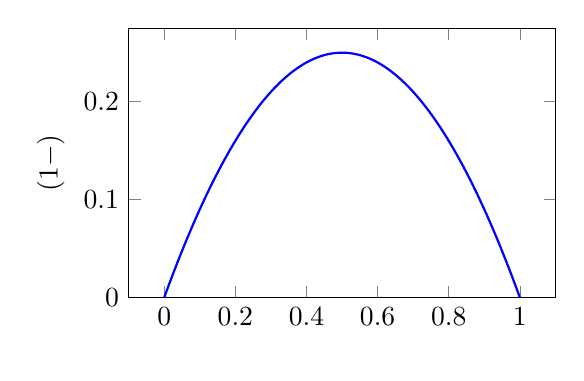
\begin{tikzpicture}
                \begin{axis}
                    [width=7cm,height=5cm,domain=0:1,samples=100,xlabel={$\param$},ylabel={$\param(1-\param)$},ymin=0]
                    \addplot[thick,blue] {x*(1-x)};
                \end{axis}
            \end{tikzpicture}\label{fig:figure6}
        \end{figure}

        \item Die \gls{Risikofunktion} des \gls{Schätzer}s $t$ ist gegeben durch die Abbildung $\param\mapsto\dfrac{\param(1-\param)}{n}$.
        \item Wir wollen nun den \gls{Schätzer} $t$ mit einem anderen \gls{Schätzer} vergleichen.
        Sei der \gls{Schätzer} $\tilde t$ gegeben durch
        \[
            \tilde t(x) = \frac{x_1+x_n}{2} \qquad \text{für alle } x\in\{0,1\}^n ,
        \]
        das heißt, wir sind ``faul'' und verwenden nur den ersten und den letzten Stichprobenwert.
        Das Risiko von $\tilde t$ in $\param$ ist gegeben durch $R(\param,\tilde t) = \dfrac{\param(1-\param)}{2}$ (dieselbe Rechnung wie für $t$, nur diesmal mit Stichprobengröße $2$).

        Wir haben das -- keineswegs überraschende -- Ergebnis, dass $t$ mindestens so gut ist wie $\tilde t$, sofern $n\geq2$.
        Für $n>2$ haben wir sogar, dass $t$ besser als $\tilde t$ ist.
    \end{enumerate}
\end{bsp}

\begin{lem}
    \textbf{Rechenregeln für Bias und Risiko} \txc{(Skript 26)} \\
    Sei $t$ ein \gls{Schätzer} für $g(\param)$.
    Dann gelten:
    \begin{enumerate}[label=(\alph*)]
        \item Der \gls{Schätzer} $t$ ist genau dann erwartungstreu, wenn $\ET[T]=g(\param)$ für alle $\param\in\praum$ gilt.
        \item $R(\param,t) = (\mathrm{Bias}_t(\param))^2 + \mathrm{Var}_\param(T)$
        \item Ist $t$ erwartungstreu, so gilt $R(\param,t) = \mathrm{Var}_\param(T)$.
    \end{enumerate}

    \paragraph{Beweis.}
    \begin{enumerate}[label=(\alph*)]
        \item Folgt direkt aus der Definition des Bias und der Erwartungstreue.
        \item Aus der Definition von Bias und Risiko folgt mit Hilfe einer Nullergänzung, dass
        \begin{align*}
            R(\param,t) &= \ET\big[(T-g(\param))^2\big] = \ET\Big[\big((T-\ET[T])+(\ET[T]-g(\param))\big)^2\Big] \\
            &= \ET\big[(T-\ET[T])^2\big] + 2\big(\ET[T]-g(\param)\big)\,\ET\big[T-\ET[T]\big] + \big(\ET[T]-g(\param)\big)^2 \\
            &= \mathrm{Var}_\param(T) + (\mathrm{Bias}_t(\param))^2 \cdot
        \end{align*}
        \item Folgt direkt aus der Definition der Erwartungstreue. \qedhere
    \end{enumerate}
\end{lem}

Bisher haben wir ausschließlich den Parameter geschätzt, der im Spezialfall der \gls{Bernoulli-Variable}n mit dem Erwartungswert zusammenfällt.
Im allgemeinen Fall, wenn die \gls{Stichprobenvariable}n möglicherweise eine andere Verteilung haben, dient das
arithmetische Mittel als \gls{Schätzer} für den Erwartungswert.
Wir sehen uns als Nächstes ein paar Beispiele an.
Der allgemeine Fall verbleibt als Hausaufgabe.

\begin{bsp}
    \textbf{Das arithmetische Mittel als \gls{Schätzer} des Erwartungswerts} \txc{(Skript 26)} \\
    Seien $X_1,\dots,X_n$ \gls{Stichprobenvariable} und $t$ ein \gls{Schätzer} für den Erwartungswert, der durch
    \[
        t(x) = \bar x = \frac1n\sum_{i=1}^n x_i \qquad \text{für alle } x\in\spr
    \]
    definiert ist.

    \begin{enumerate}[label=(\alph*)]
        \item \textbf{Geometrisch verteilte Stichprobenvariable.} Sei $\param\in\praum=[0,1]$ und gelte
        \[
            \pe_{\param}(X_i=k) = (1-\param)^{k-1}\param \qquad \text{für alle } k\in\nz \cdot
        \]
        Dann ist der Bias des \gls{Schätzer}s $t$ gegeben durch
        \[
            \mathrm{Bias}_t(\param) = \ET\left[\frac1n\sum_{i=1}^n X_i\right] - \E[X_1] = \frac1n\sum_{i=1}^n \ET[X_i] - \E[X_1] = 0 \qquad \text{für alle } \param\in\praum ,
        \]
        weil $X_1,\dots,X_n$ identisch verteilt sind.
        Wir schätzen mit $t$ den Erwartungswert $\E[X_1]=\frac1\param$.
        Der \gls{Schätzer} ist erwartungstreu.

        \item \textbf{Gleichverteilte Stichprobenvariable.} Sei $\param\in\praum=\nz$ und gelte
        \[
            \pe_{\param}(X_i=k) = \frac1\param \qquad \text{für alle } k\in\{1,\dots,\param\} \cdot
        \]
        Dann ist der Bias des \gls{Schätzer}s $t$ gegeben durch
        \[
            \mathrm{Bias}_t(\param) = \ET\left[\frac1n\sum_{i=1}^n X_i\right] - \ET[X_1] = 0 \qquad \text{für alle } \param\in\praum ,
        \]
        weil $X_1,\dots,X_n$ identisch verteilt sind.
        Wir schätzen mit $t$ den Erwartungswert $\ET[X_1]=\frac{\param+1}{2}$.
        Der \gls{Schätzer} ist erwartungstreu.

        \item \textbf{Poisson-verteilte Stichprobenvariable.} Sei $\param\in\praum=\nz$ und gelte
        \[
            \pe_{\param}(X_i=k) = \frac{\param^k}{k!}e^{-\param} \qquad \text{für alle } k\in\nz_0 \cdot
        \]
        Dann ist der Bias des \gls{Schätzer}s $t$ gegeben durch
        \[
            \mathrm{Bias}_t(\param) = \ET\left[\frac1n\sum_{i=1}^n X_i\right] - \ET[X_1] = 0 \qquad \text{für alle } \param\in\praum ,
        \]
        weil $X_1,\dots,X_n$ identisch verteilt sind.
        Wir schätzen mit $t$ den Erwartungswert $\ET[X_1]=\param$.
        Der \gls{Schätzer} ist erwartungstreu.
    \end{enumerate}
\end{bsp}

Wir können auch Funktionen des Parameters schätzen.
Wir betrachten hier exemplarisch die Varianz als eine solche Funktion.

\begin{bsp}
    \textbf{\gls{Schätzer} für die Varianz} \txc{(Skript 26)} \\
    Seien $X_1,\dots,X_n$ unabhängige \gls{Stichprobenvariable}\footnote{Wir nehmen nicht an, dass die Stichprobenvariablen \gls{Bernoulli-Variable} sind.} und $t$ ein \gls{Schätzer} für den Erwartungswert, der durch
    \[
        t(x) = \bar x = \frac1n\sum_{i=1}^n x_i \qquad \text{für alle } x\in\spr
    \]
    definiert ist.

    Eine naheliegende Idee ist es, analog zur Stichprobenvarianz, die Abbildung $s^2$ mit
    \[
        s^2(x) = \frac1n\sum_{i=1}^n (x_i-\bar x)^2 = \frac1n\sum_{i=1}^n \left(x_i - \frac1n\sum_{j=1}^n x_j\right)^2 \qquad \text{für alle } x\in\spr
    \]
    zu wählen.

    Ist dieser \gls{Schätzer} erwartungstreu?

    Wir können uns die (Schreib-)Arbeit etwas erleichtern, wenn wir annehmen, dass $\ET[X_i]=0$ gilt.
    Diese Annahme bedeutet keine Einschränkung der Allgemeingültigkeit des herzuleitenden Resultats, wie wir mittels einer Nullergänzung leicht sehen:
    \begin{align*}
        X_i - t(X) &= (X_i-\ET[X_i]) + \left(\ET[X_1] - \frac1n\sum_{i=1}^n X_i\right) \\
        &= (X_i-\ET[X_i]) - \left(\frac1n\sum_{i=1}^n (X_i-\ET[X_i])\right) \\
        &= (X_i-\ET[X_i]) - t\big((X_1-\ET[X_1],\dots,X_n-\ET[X_n])\big) \cdot
    \end{align*}
    Das heißt, $X_i-t(X)$ hängt nicht vom Erwartungswert der \gls{Stichprobenvariable}n ab.

    Im Folgenden nehmen wir also an, dass $\ET[X_i]=0$ gilt.
    Umschreiben zeigt:
    \[
        s^2(X) = \frac1n\sum_{i=1}^n\Big[X_i^2 - 2X_i t(X) + (t(X))^2\Big] = \frac1n\sum_{i=1}^n X_i^2 - 2(t(X))^2 + (t(X))^2 = \frac1n\sum_{i=1}^n X_i^2 - (t(X))^2 \cdot
    \]
    Daher gilt
    \[
        \ET\big[s^2(X)\big] = \frac1n\sum_{i=1}^n \ET[X_i^2] - \ET\big[(t(X))^2\big] = \ET[X_1^2] - \ET\big[(t(X))^2\big] = \ET[X_1^2] - \frac{1}{n^2}\sum_{i,j=1}^n \ET[X_i X_j] \cdot
    \]
    Für $i\neq j$ gilt aufgrund der Unabhängigkeit von $X_i$ und $X_j$, dass $\ET[X_i X_j] = \ET[X_i]\,\ET[X_j] = 0$.
    Daher bleiben von der Doppelsumme nur die Diagonalterme, das heißt,
    \[
        \ET\big[s^2(X)\big] = \ET[X_1^2] - \frac{1}{n^2}\sum_{i=1}^n \ET[X_i^2] = \ET[X_1^2] - \frac1n\ET[X_1^2] \cdot
    \]
    Da wir angenommen haben, dass $\ET[X_1]=0$ gilt, folgt
    \[
        \ET\big[s^2(X)\big] = \left(1-\frac1n\right)\mathrm{Var}_\param(X_1) \cdot
    \]
    Wir sehen somit, dass $s^2$ \emph{kein} erwartungstreuer \gls{Schätzer} der Varianz ist.
    Wir sehen aber auch, dass der Unterschied nur im Vorfaktor $1-\frac1n$ liegt.
    Wenn wir $s^2$ mit $\frac{n}{n-1}$ multiplizieren, erhalten wir einen erwartungstreuen \gls{Schätzer}.
    In der Tat definiert
    \[
        \widehat\sigma^2(x) = \frac{1}{n-1}\sum_{i=1}^n (x_i-\bar x)^2 \qquad \text{für alle } x\in\spr
    \]
    einen erwartungstreuen \gls{Schätzer} für die Varianz, wenn der Erwartungswert unbekannt ist und daher durch den \gls{Schätzer} $\bar x$ ersetzt werden muss.
\end{bsp}
